
\chapter{Immersed Boundary Methods for No-Slip Walls}
\section{Overview of Immersed Boundary Methods}

\begin{figure}[!bp]
  \centering
  \subfloat[cartesian grid]{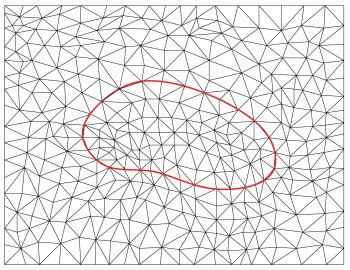
\includegraphics[width=0.4\textwidth]{gfx/immersed_boundary_methods/general_partition_triangle.jpg}\label{fig:grid_f1}}
  \hfil
  \subfloat[unstructured body-fitted grid]{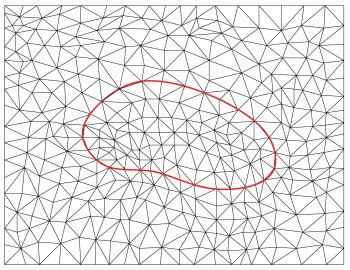
\includegraphics[width=0.4\textwidth]{gfx/immersed_boundary_methods/general_partition_triangle.jpg}\label{fig:grid_f2}}
  \caption{Different types of numerical grids}
\end{figure}

For many fluid problems it is mandatory to solve the equations of motion with respect to complex-shaped geometries \.
The algorithm introduced in section () is not yet suitable for such a scenario.
For instance the simulation inside a spheric geometry is impossible, since the boundaries
do not coincide with the implemented cartesian grid. Nevertheless there exist different approaches to overcome this problem,
which shall be introduced here. \\
The common approach to extend the algorithm would be to use a body-fitted mesh (see figure \ref{fig:grid_f1}),
different advantages and disadvantages arise with this kind of implementation (see \citep{Mittal2005}).
One benefit is a much simpler deployment of the desired boundary condition, due to the overlap of the grid with domain border.
Furthermore a higher accuracy can be achieved \citep{Gornak2013}.
However, using an unstructered grid generates plenty of computational overhead, during and before the execution of a simulation.
The generation of the grid is very complicated in contrast to using a cartesian grid, this can be even more complicated when
considering moving boundaries.
Also solving the finite differenc schemes on a curvilinear coordinate system, leads to more calculations on a single grid point.
The last important aspect is the implementation on the gpu.
Like discussed in section () it is more efficient to use homogenous storage and calculation pattern on a CUDA-device,
the use of unstructured data makes this very difficult.
Altough some attempts exists to solve these difficulties (see i.e. PAP), it is still uncertain if the obtained performance loss would be acceptable.\\
A set of alternative methods, to resolve the problems described above, are so called Immersed Boundary Methods.
The term was first mentioned in (PESKIN 1972), for the simulation of blood flow through a heartvale, but has since then been used for a variety of
methods (MITTAL).  All of them have the idea in common to perform the simulations on a cartesian grid which does not conform to the domain boundary.
To satisfy the desired boundary conditions additional terms are introduced into the equations of motion.
In general one can distinguish between contiuous forcing methods and direct forcing methods.
Continious forcing methods try to mimic the boundary using a localized force which acts on the boundary,
since the surface is tracked by lagrangian points this methods can be well suited for moving boundaries (MITTAL).
One common problem is that continous forcing can arise to stability problem and numerical oscillations in numericial stiff problem (SOURCE).
The direct forcing approach tries to satisfies the boundary condition, by imposing it directly to points near the fluid surface for example
trough an interpolaltion procedure.
Some of the major drawbacks using the IBM is the loss in  spatial accuracy at the boundary, therefore it can be necessary to use a higher grid resolution
compared to a body-fitted mesh.  Futhermore the non-conforming (?) boundaries are more difficult implement.
The benefits of these methods is the use of a cartesian grid, which is much more suited for a gpu-based implementation (see section X).
As a result the overall performance will probably be in the same order as the original algorithm.
In the thesis the Implementation of different Immersed Boundary Methods is seperated into three chapters depending on the boundary condition and application.
This chapter beginns with Implementation of NoSlip-Walls which are the easisest to implement.
The term Immersed Boundary Method is vaguely defined in literature, in this thesis we refer to it with all methods introduced in the following three chapters.


\section{Implemented IBMs}
\subsection{Volume Penalization}
\subsection{Direct Forcing}
\subsection{Volume fraction}
\subsection{Interpolation}
\newpage

\section{Validation}

In order to ensure a correct numerical behaviour of the introduced methods,
a large part of the thesis deals with the numerical validation.
Multiple examples from simple to more complex testcases are introduced in this section.
In general it is necessary to obtain a good evaluation of the numerical truncation error, the numerical stability over longer periods of time
and the fullfilment of the conversation laws, most importantly mass conservation.
Grid convergence studys against theoretical and high-resolution numerical solutions  will be performed
and compared for the different IBMs.


\subsection{Laminar Poiseuille-Flow}

\begin{figure}[!bp]
  \centering
  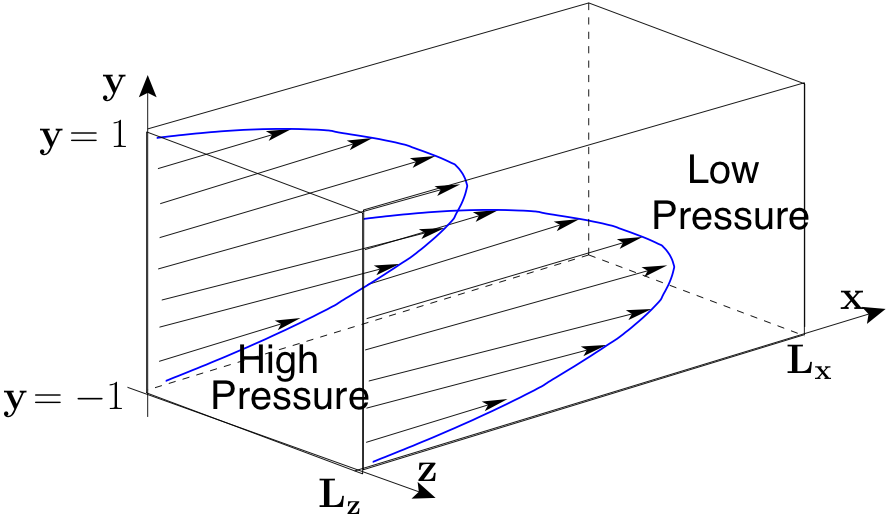
\includegraphics[width=0.8\textwidth]{gfx/immersed_boundary_methods/val_volpen/poiseuilleflow.png}\label{b}
  \caption{Theoretical setup of the poiseuille-flow channel.}
\end{figure}

%\begin{wrapfigure}{r}{0.5\textwidth}
%  \begin{center}
%      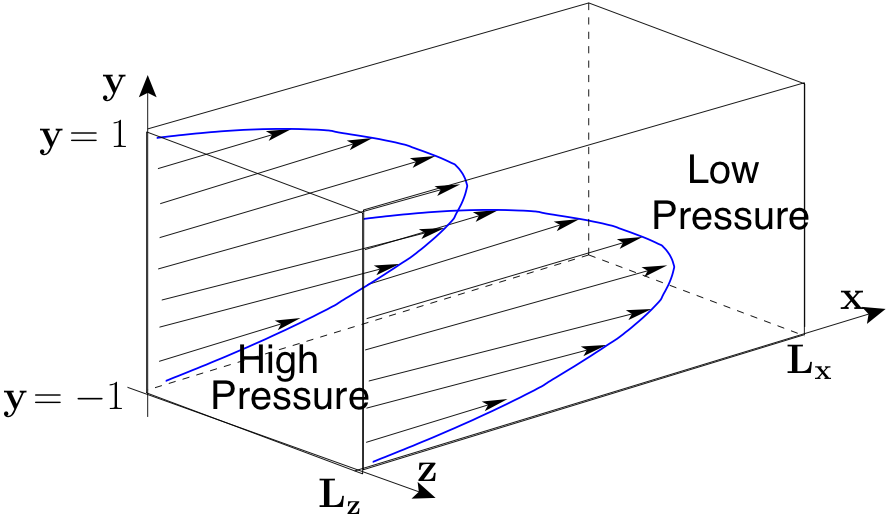
\includegraphics[width=0.48\textwidth]{gfx/immersed_boundary_methods/val_volpen/poiseuilleflow.png}
%   \end{center}
%          \caption{ paxvleb xvle}
%\end{wrapfigure}


The first testcases is the laminar poiseuille-flow, the theoretical setup is presented in figure ().
It consist of two infintiy long planes at $z=h_1$ and $z=h_2$, which are oriented parallel to the xy-plane and the distance $\Delta h = h_2 - h_1$ between them.
Numerically this is realized by using periodic boundaries in xy-direction and no-slip boundaries in z-direction.
The velocity profile results from an external force, given by a  pressure gradient in x-direction, which is introduced into the naviers-stokes equation.
No other forces are present furthermore the flow will be independent of the y coordinate,
hence for the steady state $\partial v_x /\partial t = 0$ the equations of motion can be reduced to:

\begin{align}
\frac{\partial v_x}{\partial t} &= - \frac{\partial p}{\partial x} + D \frac{\partial^2 v_x}{\partial z^2} = 0
\end{align}

The equation can simply be integrated twice which yields the solution

\begin{align}
v_x &= \frac{1}{2D}\frac{\partial p}{\partial x}z^2 + zc_1 + c_2
\end{align}

Using the noslip-boundary condition $v_x(h_1) = v_x(h_2) = 0$ and furthermore by defining
$A:=\frac{1}{2D}\frac{\partial p}{\partial x}$ one obtains the additional conditions

\begin{align}
c_1 &= A\frac{h_1^2 -h_2^2}{h_2 - h_1} = -A(h_1+h_2)\\
c_2 &= A(h_1(h_1 + h_2) - h_1^2) = Ah_1h_2\\
\end{align}

The velocity is than given by the quadratic function

\begin{align}
v_x &= A(z^2 - z(h_1 + h_2) + h_1h_2)
\end{align}

The maximum velocity and postinon can be obtained by simple calculus

\begin{align}
z_{max} &= \frac{h_1+h_2}{2} \wedge v_{max} = A\left(h_1h_2 - \frac{(h_1 + h_2)^2}{4}\right)
\end{align}

With the given theoretical solution, the next objective is the comparison
to the default implementation, the volume penalization method and the direct forcing method.
Since we have a flow parallel to the grid  it does not make sence to compare it to the interpolation methods
In the default setup the noslip-boundaries are realized with the default implementation, like explained in section ().
For the immersed boundary methdos the upper- and lower boundaries are given by the masking function.

\begin{align}
H(x, y, z) = \begin{cases}
                    0, & \text{for \  }  z < h_2 \wedge z>h_1 \\
                    1, & \text{else}.
             \end{cases}
\end{align}

For the comparision with a theoretical solution it is necessary to ensure that the surface grid points match with the total height $h$ of the channel.
This can be ensured with






For the comparison of the



all directions and no-slip b.
The

The setup is given by two inifinity long  parallel pla



Die Volume-Penalization Methode ermöglicht es, durch einen Kraftterm der auf die einzelnen Fluidzellen wirkt, mit wenig Aufwand Noslip-Ränder zu implementieren.
Das Verfahren wurde in mehreren Publikationen z.B. [bla] erfolgreich verwendet, eine mathematisch exaktere Abhandlung lässt sich z.B. in [bla2] finden.

\begin{wrapfigure}{r}{0.5\textwidth}
  \begin{center}
  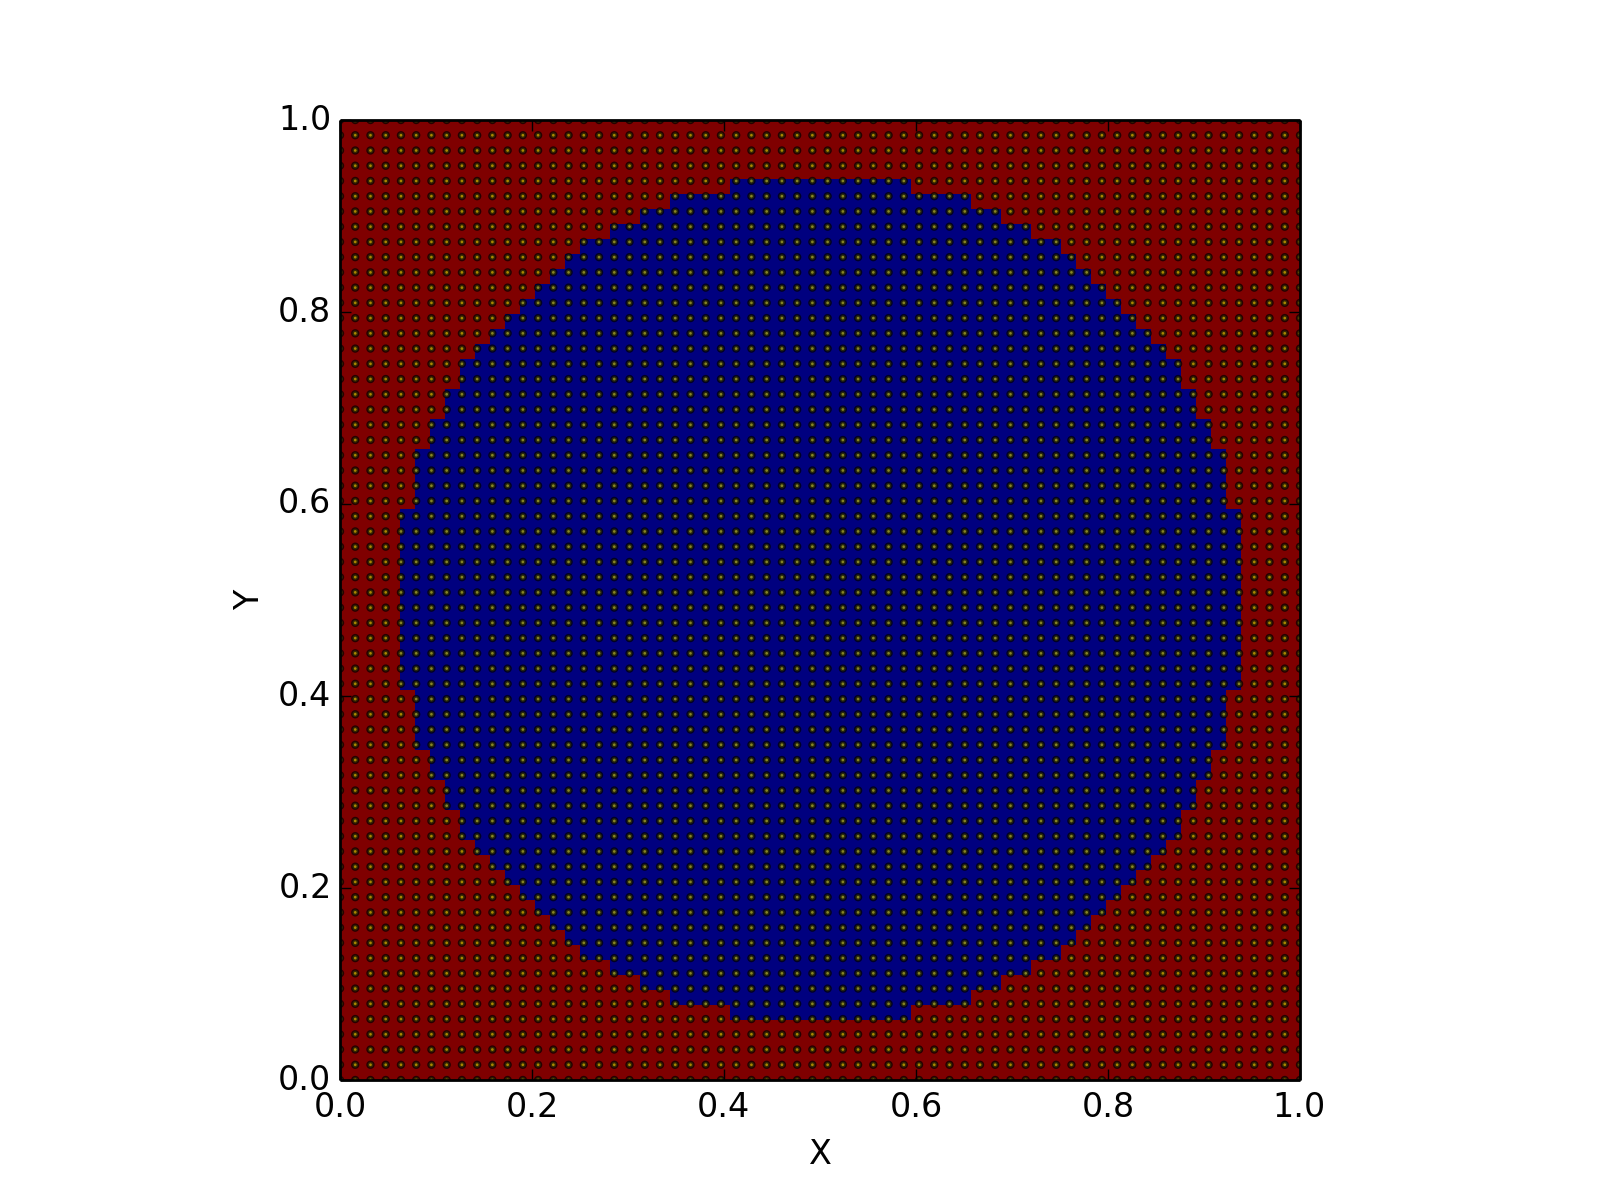
\includegraphics[width=0.5\textwidth]{gfx/immersed_boundary_methods/mask.png}\label{fig:mask_vp}
  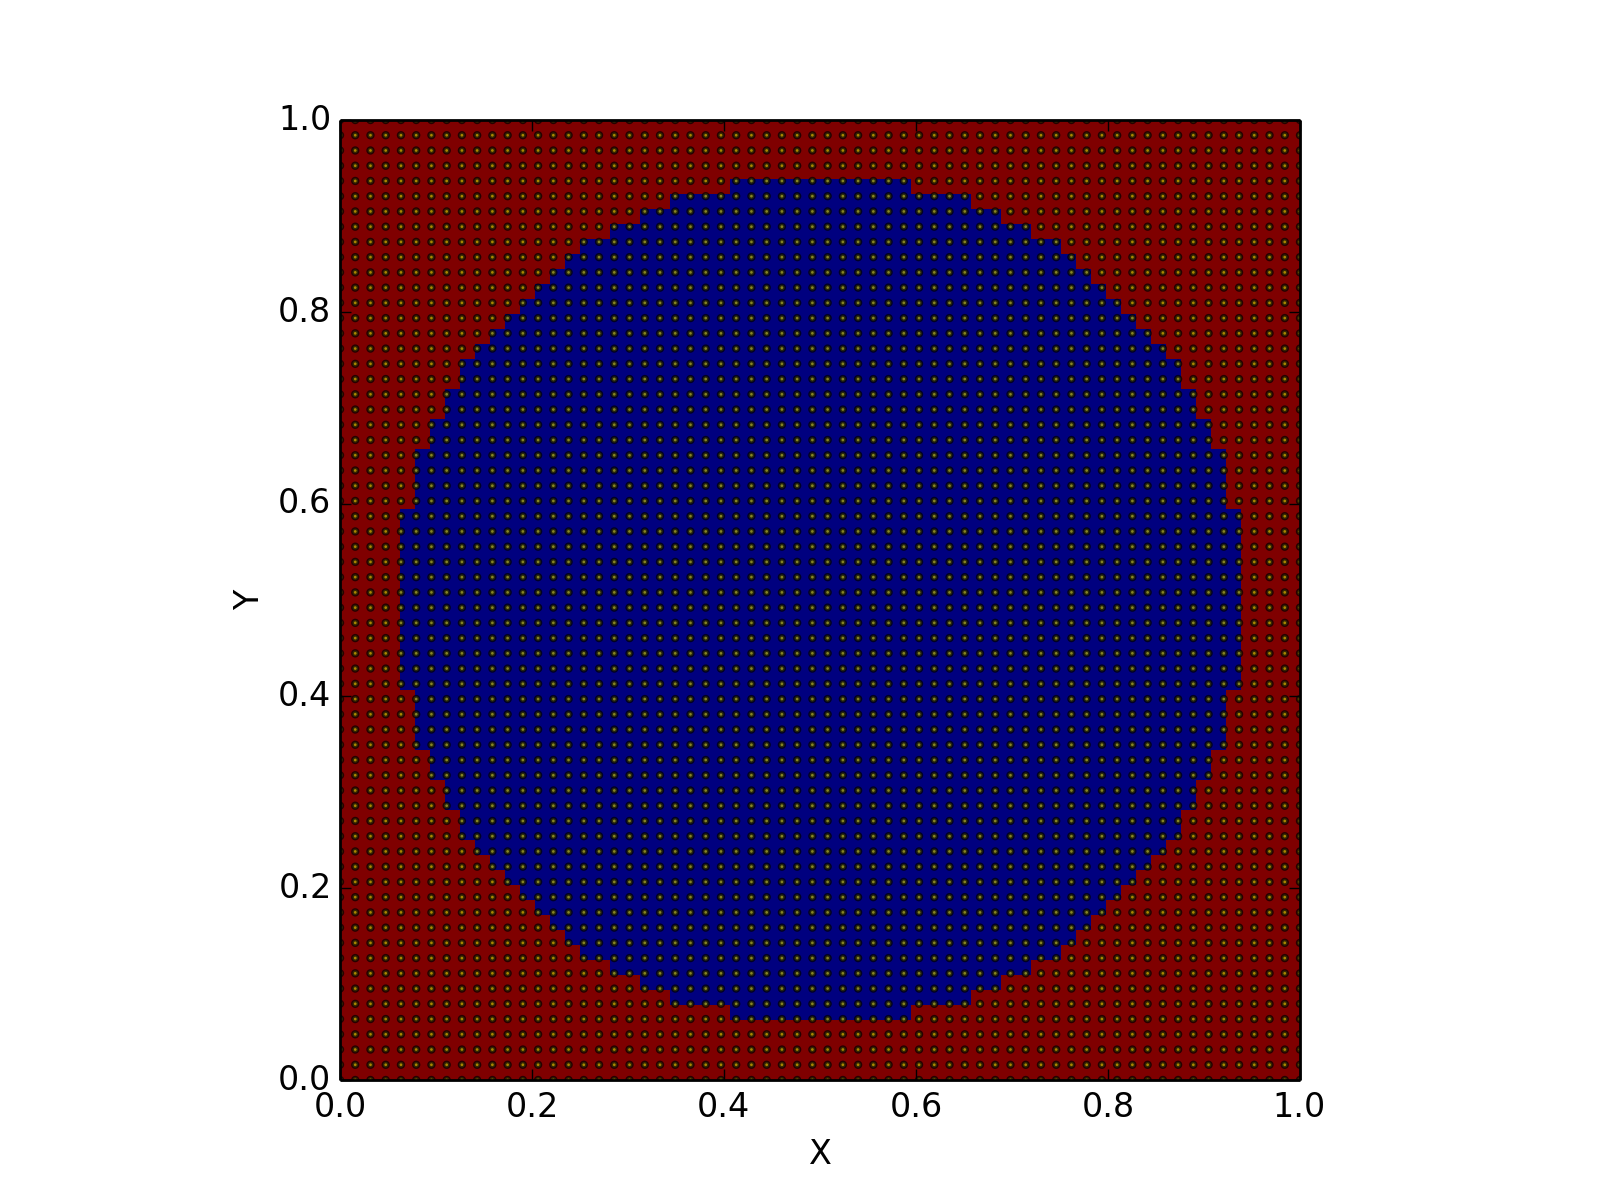
\includegraphics[width=0.5\textwidth]{gfx/immersed_boundary_methods/mask.png}\label{fig:mask_vp}
  \end{center}
  \caption{Maskierungsfunktion $H(x,y,z=const.) = x^2 + y^2 < c$ für einen Zylinder. }
\end{wrapfigure}

Das Volumen wird zunächst in einen Fluidbereich und einen festen Wandbereich, wie in Abb.1 dargestellt, unterteilt. Für die Differenzierung der Bereiche während der Simulation wird  eine Maskierungsfunktion
\begin{align}
H(x, y, z) = \begin{cases}
                    0, & \text{für } \vec{x}(x,y,z) \in Fluid, \\
                    1, & \text{sonst}.
             \end{cases}
\end{align}
verwendet. Als zusätzlicher Kraftterm wird nun eine exponentielle Dämpfung eingeführt die nur auf den Wandbereich des Volumens wirkt.
\begin{align}
\vec{f} = \frac{H(x, y, z)}{\nu}(\vec{v} - \vec{v_0})
\end{align}
Bei $\vec{v_0}$ handelt es sich um die gewünschte Randbedingung, der Kraftterm ist also proportional zur Auslenkung $\vec{v}$ eines Punktes vom gewünschten Ruhezustand.
Die Antwort des Kraftterms wird durch die Dämpfungrate $\nu$ reguliert. Je kleiner $\nu$ desto stärker ist die Dämpfungsrate, allerdings kann der Term
nicht beliebig klein gesetzt werden da die Stabilität für $\nu < dt$ nicht mehr gewährleistet ist [source].
Da für die Lösung der der Geschwindingskeitsfelder mit der Methode der künstliche Kompressibilität  bereits ein sehr kleiner Zeitschritt verwendet wird (s.Abb. X)
kann im Vergleich zu anderen Verfahren wie z.B. (pseudo-spektrale) eine relativ starke Dämpfungsrate verwendet werden.

\subsubsection{Validierung mit MASA}
-validierung mit masa für alle verfahren oben.. cube /evtl zylinder?
-vegl. und argumentation ränder ehh auf null.
-ein beispiel mit vol.pen.

\subsubsection{Validierung : planare Poiseuille Strömung}
Es stellt sich die Frage in welcher Größenordnung die Dämpfungskonstante $\nu$ der Volume Penalization methode liegen muss, um einen möglichst kleinen
Fehler zu gewährleisten. Ein einfacher Testfall der sich hierfür betrachen lässt ist eine einfache planare poiseuille strömung, diese ist schematisch in Abb. (x). dargestellt.
\paragraph*{Theoretische Beschreibung}\mbox{}\\
Wir betrachten eine laminare Strömung in x-Richtung die durch einen Druckgefälle $f=-\frac{\partial p}{\partial x}$ angetrieben wird.
Für die x- und y-Richtung werden periodische Randbedingungen angenommen. In z-Richtung wird das Volumen durch zwei Ebenen bei $h_1$ und $h_2$ begrenzt,
es gilt $ \vec{v}(z=h_1) = \vec{v}(z=h_2) = 0$.
Im stationären Fall lässt sich  die Bewegungsgleichung dann  auf eine Dimension reduzieren, es gilt:

Für die Strömung lässt sich die Reynoldszahl dann gemäß $Re \propto \frac{v_{max}}{D}$  bestimmen.
\begin{figure}[!hbtp]
  \centering
  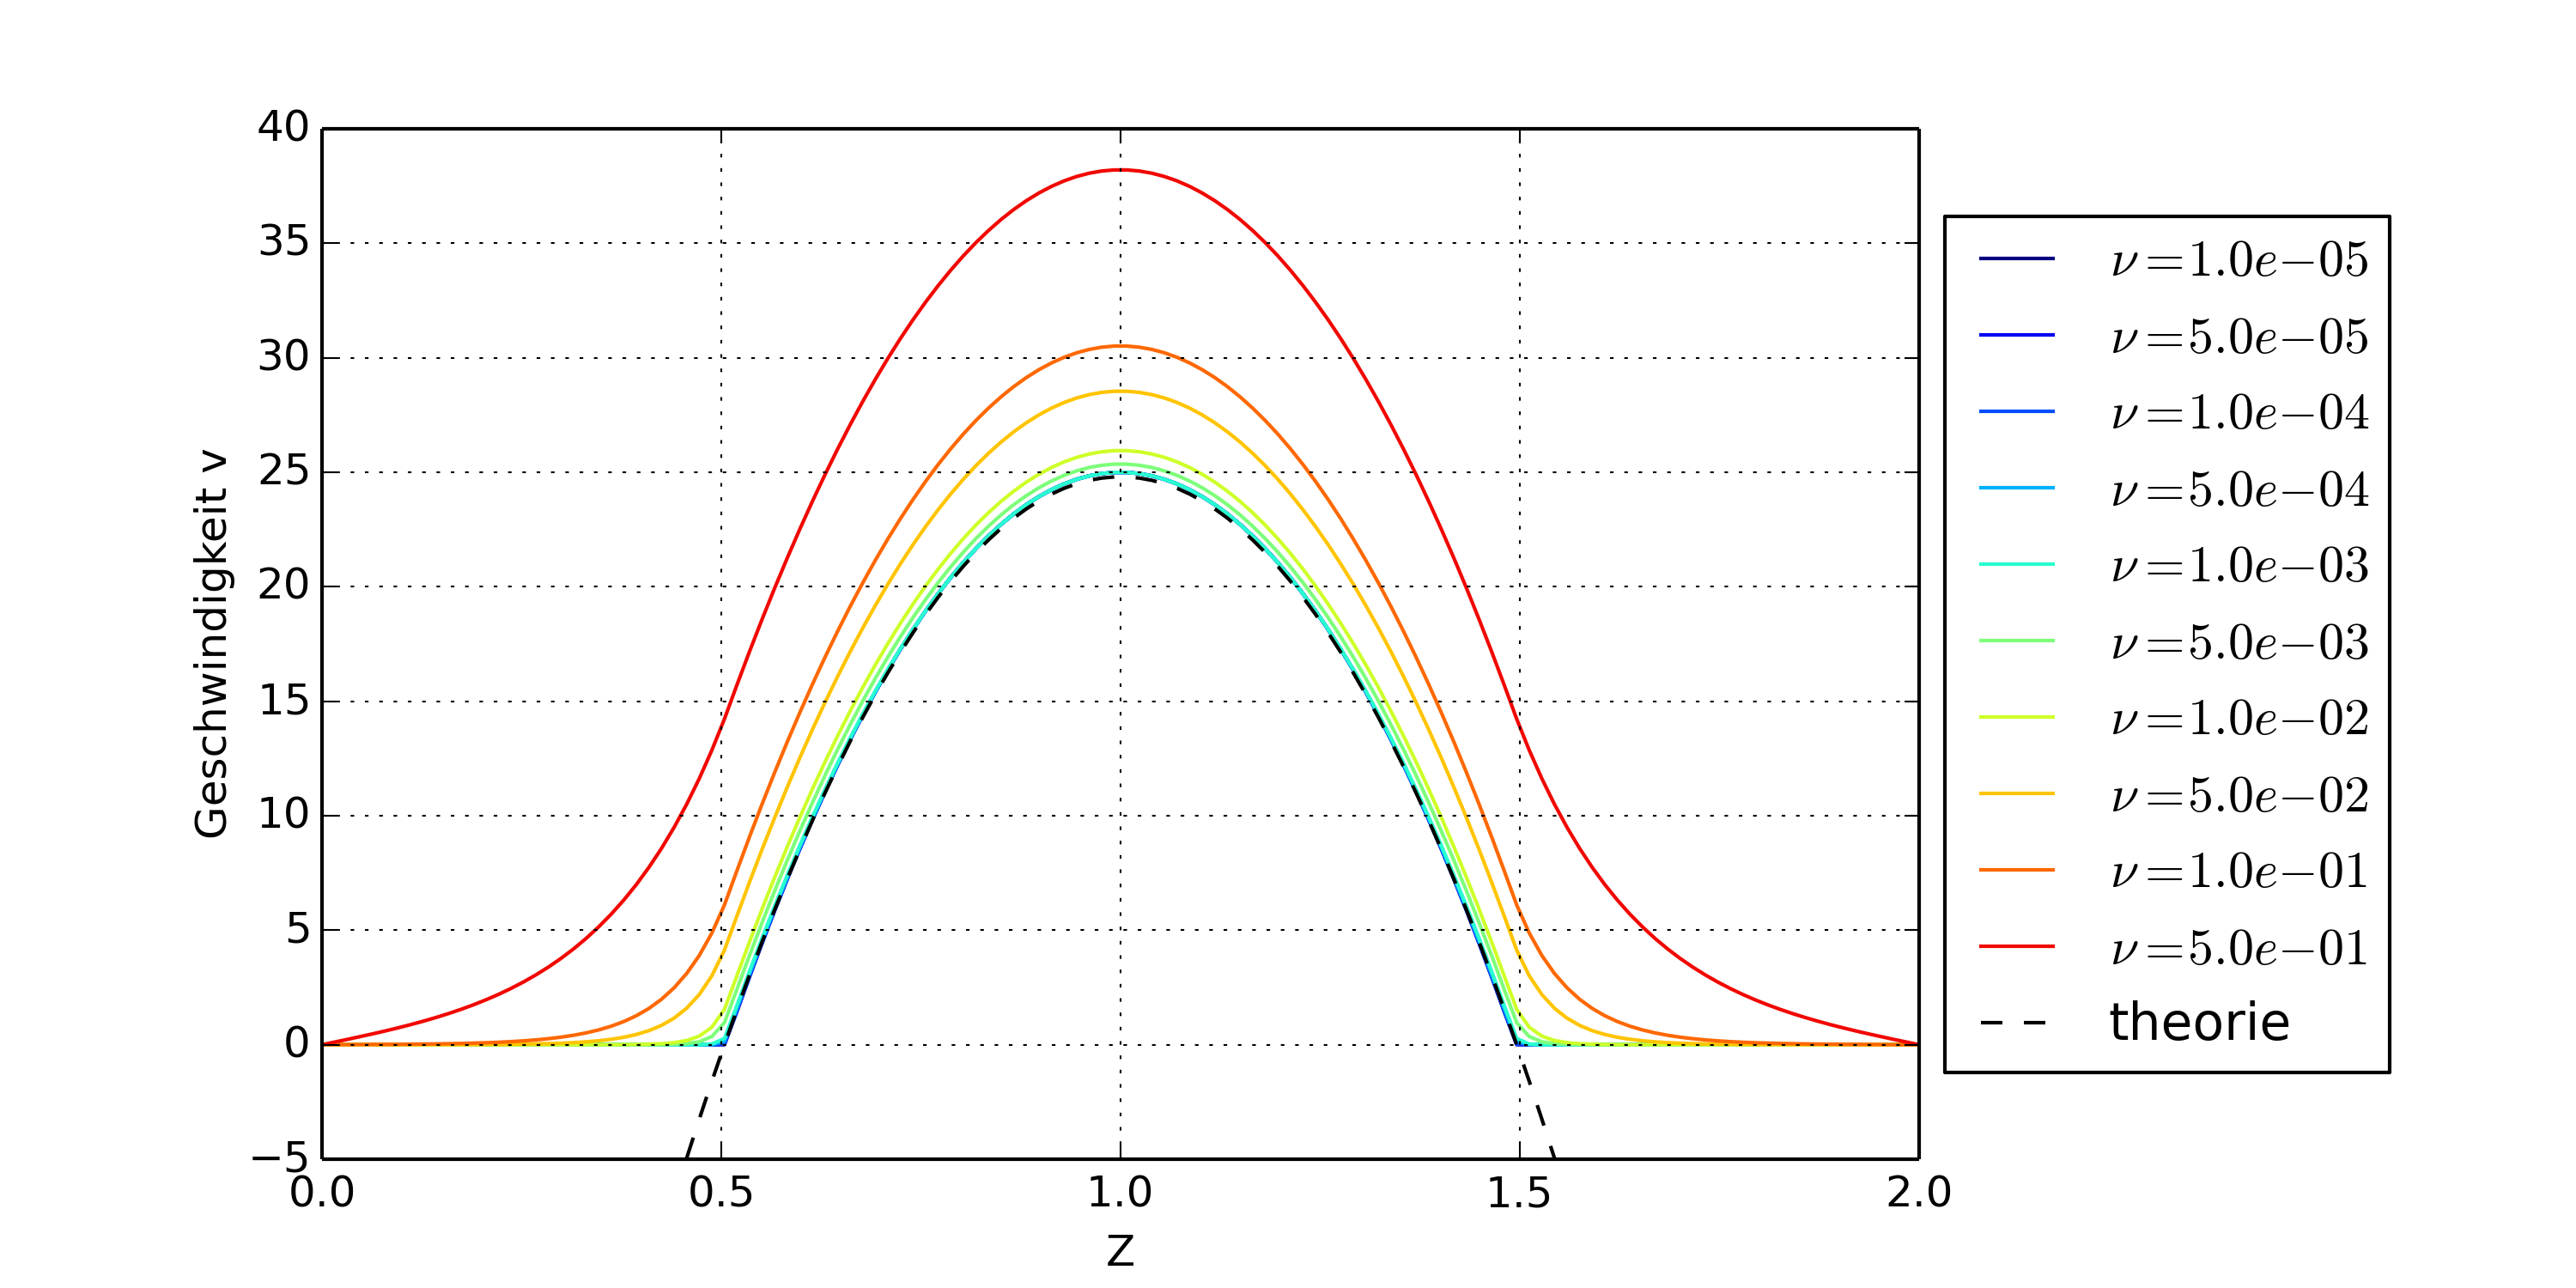
\includegraphics[width=0.9\textwidth]{gfx/immersed_boundary_methods/vp_flow.png}\label{fig:vp_flow}
  \caption{Geschwindigkeistprofile im Kanal bei Variation der Dämpfungskonstante $\nu$ und Reynoldszahl $Re=500$.}
\end{figure}

\paragraph*{Setup}\mbox{}\\
Um die Abhängigkeit des Fehlers von der Dämpfungskonstante zu betrachten wurde ein Kanal mit $l_x=1$, $l_y=1$ und $l_z=2$ sowie $h_1=0.25$, $h_2=0.75$.
betrachtet. Die Maskierungsfunction ergibt sich damit gemäß $H(z) = (z>h1) \wedge (z<h2)$.
Für die Reynoldszahl wurden Werte im Intervall $Re \in [100, 500]$ verwendet, die Dämpfungskonstante wurde zwischen $\nu \in [1e-5, 0.1]$ variert, während der Zeitschritt mit $dt =1e-5$ konstant gehalten wurde. Die genauen Angaben für alle Parameter sind in (Anhang Tab.X) zu finden.

\paragraph*{Ergebnisse}\mbox{}\\
Zunächst ist in Abb. \ref{fig:vp_flow} das Geschwindigkeitsprofil der Strömung für $Re=500$ exemplarisch dargstellt. Es lässt sich bereits qualitativ sehr gut erkennen, dass für eine
starke Dämfung die Kanalströmung an den Grenzen $h_1$ und $h_2$ verschwindet und gut mit der dem theoretischen Profil übereinstimmt.
Bei einem Verringern der Dämpfungrate entwickelt sich im Rand ein Geschwindigkeitsprofil.
Um sicherzustellen dass sich das Profil vollständig entwickelt wurde die Simulation bis zu dem Zeitpunkt fortgegeführt
 in welchem die kinetische Energie des Systems einen stationären Wert erreicht. Anschließend wurde der absolute und relative Fehler mit Formel (X) berechnet,
dabei wurde das theoretische Profil gemäß () verwendet. Die Ergebnisse sind in Abbildung \ref{fig:vp_error} dargestellt.

\begin{figure}[!bp]
  \centering
  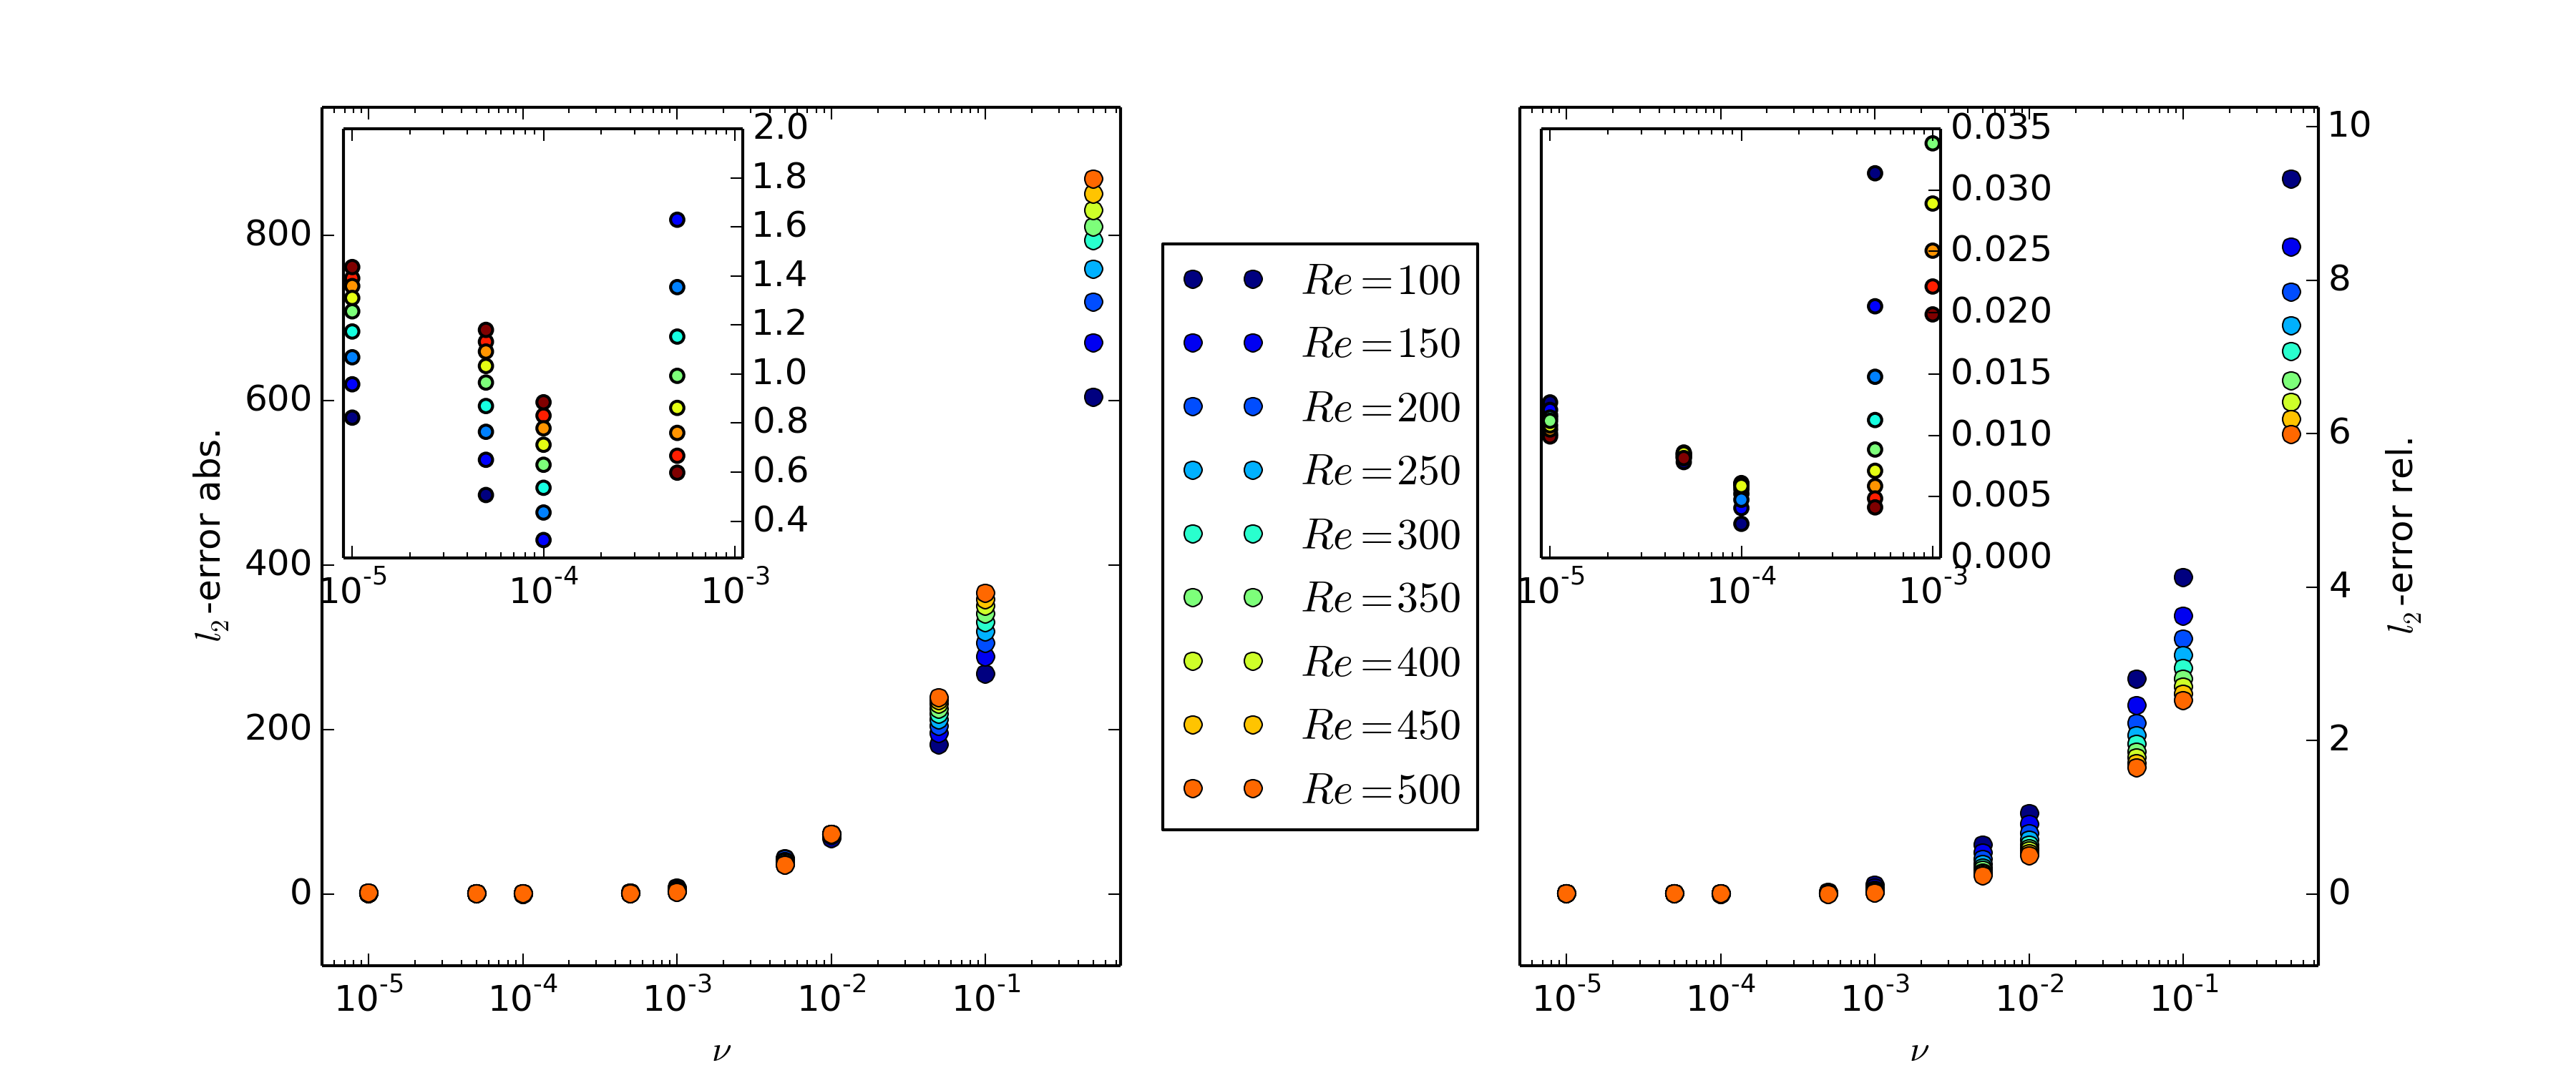
\includegraphics[width=1.0\textwidth]{gfx/immersed_boundary_methods/vp_error.png}\label{fig:vp_error}
  \caption{Absoluter und relativer Fehler in Abhängigkeit von Dämpfungskonsante $\nu$ und Reynoldszahl $Re$.}
\end{figure}

Bei beiden Fehler lässt sich ein Abfall bis $\nu=1e-4$ erkennen, anschließend kommt es zu einem minimalen Anstieg.
Betrachtet man den absoluten Fehler, so fällt auf das im Bereich $\nu>5\cdot10^{-3}$, mit steigender Reynoldszahl, der Fehler zunimmt.
Dies entspricht zunächst der Erwartung, da das Geschwindigkeitsprofil mit steigender Reynoldszahl stärker an der Wand zerrt.
Allerdings kommt es im Bereich $\nu \in [1e-3 - 1e-2]$ zu einem umgekehrten Verhalten, der Fehler nimmt mit der Reynoldszahl ab,
Du Ursache hierfür liess sich nicht eindeutig klären.
Für den relativen Fehler lässt sich ein Abfall mit steigender Reynoldszahl beobachten. Da $\vec{f} \propto (\vec{v}-\vec{v_0})  \propto Re$ wird der Reibunsterm
proportional zur Reynoldszahl skaliert. Der Fehler durch den Rand ändert sich, im Vergleich zum Geschwindigskeitsprofil kaum, wodurch der Abfall zustande kommt.
Der relative Fehler fällt bei $\nu=1e-4=10\Delta t$ auf unter 1\%, wodurch dieser Wert als geeignet angesehen werden kann für zukünftige Simulationen mit der Volume-Penalization Methode.

-todo: fluktuation im rand


\subsection{Direct Forcing Methode}
Während die Volume Penalization Methode die Geschwindigkeit ausserhalb des Volumens nicht vollständig auf Null setzt,
 kann dies durch eine implizite Berechnung des Dämpfungsterm erreichtwerden. Es stellt sich heraus das dieser Ansatz equivalent
  zu der Direct Forcing Methode ist, die erstmals von [] verwendet und in [] beschrieben wird.
Betrachten wir zunächst den diskretisierten Zeitschritt
\begin{align}
    \frac{\vec{u}^{n+1} -\vec{u}^n}{\Delta t} = \mathscr{L} + \vec{f}\\
\end{align}
wobei $\mathscr{L}$ den diskretiesierten Operatoren der PDE entspricht.
Für einen Punkt auf dem Rand des Volumens soll nun die Randbedingung $\vec{u}^{n+1} = \vec{u}_0$ eingehalten werden.
Mit Formel () folgt
\begin{align}
    \frac{\vec{u}_0 -\vec{u}^n}{\Delta t} = \mathscr{L} + \vec{f} \Rightarrow \vec{f} = \frac{\vec{u}_0 -\vec{u}^n}{\Delta t\cdot \mathscr{L}}\\
\end{align}
Mit der Annahme dass der Rand mit dem numerischen Gitter übereinstimmt ist es nicht nötig den Kraftterm zur berechnen, stattdessen lässt sich der
Schritt vereinfachen in dem der Randwert nach  jedem Zeitschritt direkt auf die gewünschte Randbedingung gesetzt wird. Durch die
implizite Behandlung kommt es zu keiner weiter Stabilitätsbedingung.
Analog zur Volume-Penalization Methode wurde eine Serie von Simulationen für eine planare Poiseuille-Strömung durchgeführt.
Das Setup enstpricht dem gleichen wie in Abschnitt (X), lediglich das Verfahren wurde entsprechend angepasst und es wurden finite Differenzen Verfahren zweiter und
vierter Ordnung getestet.
In Abbildung () ist der relative Fehler, im Vergleich zur Volume Penalization  Methode mit $\nu=1e-4$ dargestellt.
Für das Verfahren vierter Ordnung liegt der Fehler im Bereich von 1\% und ist im Mittel doppelt so groß wie für die Volume-Penalization Methode.
Der Fehler für das Verfahren zweiter Ordnung verschwindet hingegen nahezu.
Das Verhalten lässt sich durch die Verwendung unterschliedlicher Schablonen, wie in Abb() dargestellt,  der finiten differenzen Verfahren erklären.
Während das Verfahren zweiter Ordnung nur den Randpunkt sieht, liegt bei der vierten Ordnung ein Punkt innerhalb des Randes.
Da auch dieser Wert auf Null gesetzt wird, kommt es zu einem fehler in der Berechnung von $\nabla u$.

\begin{figure}[!tpb]
  \centering
  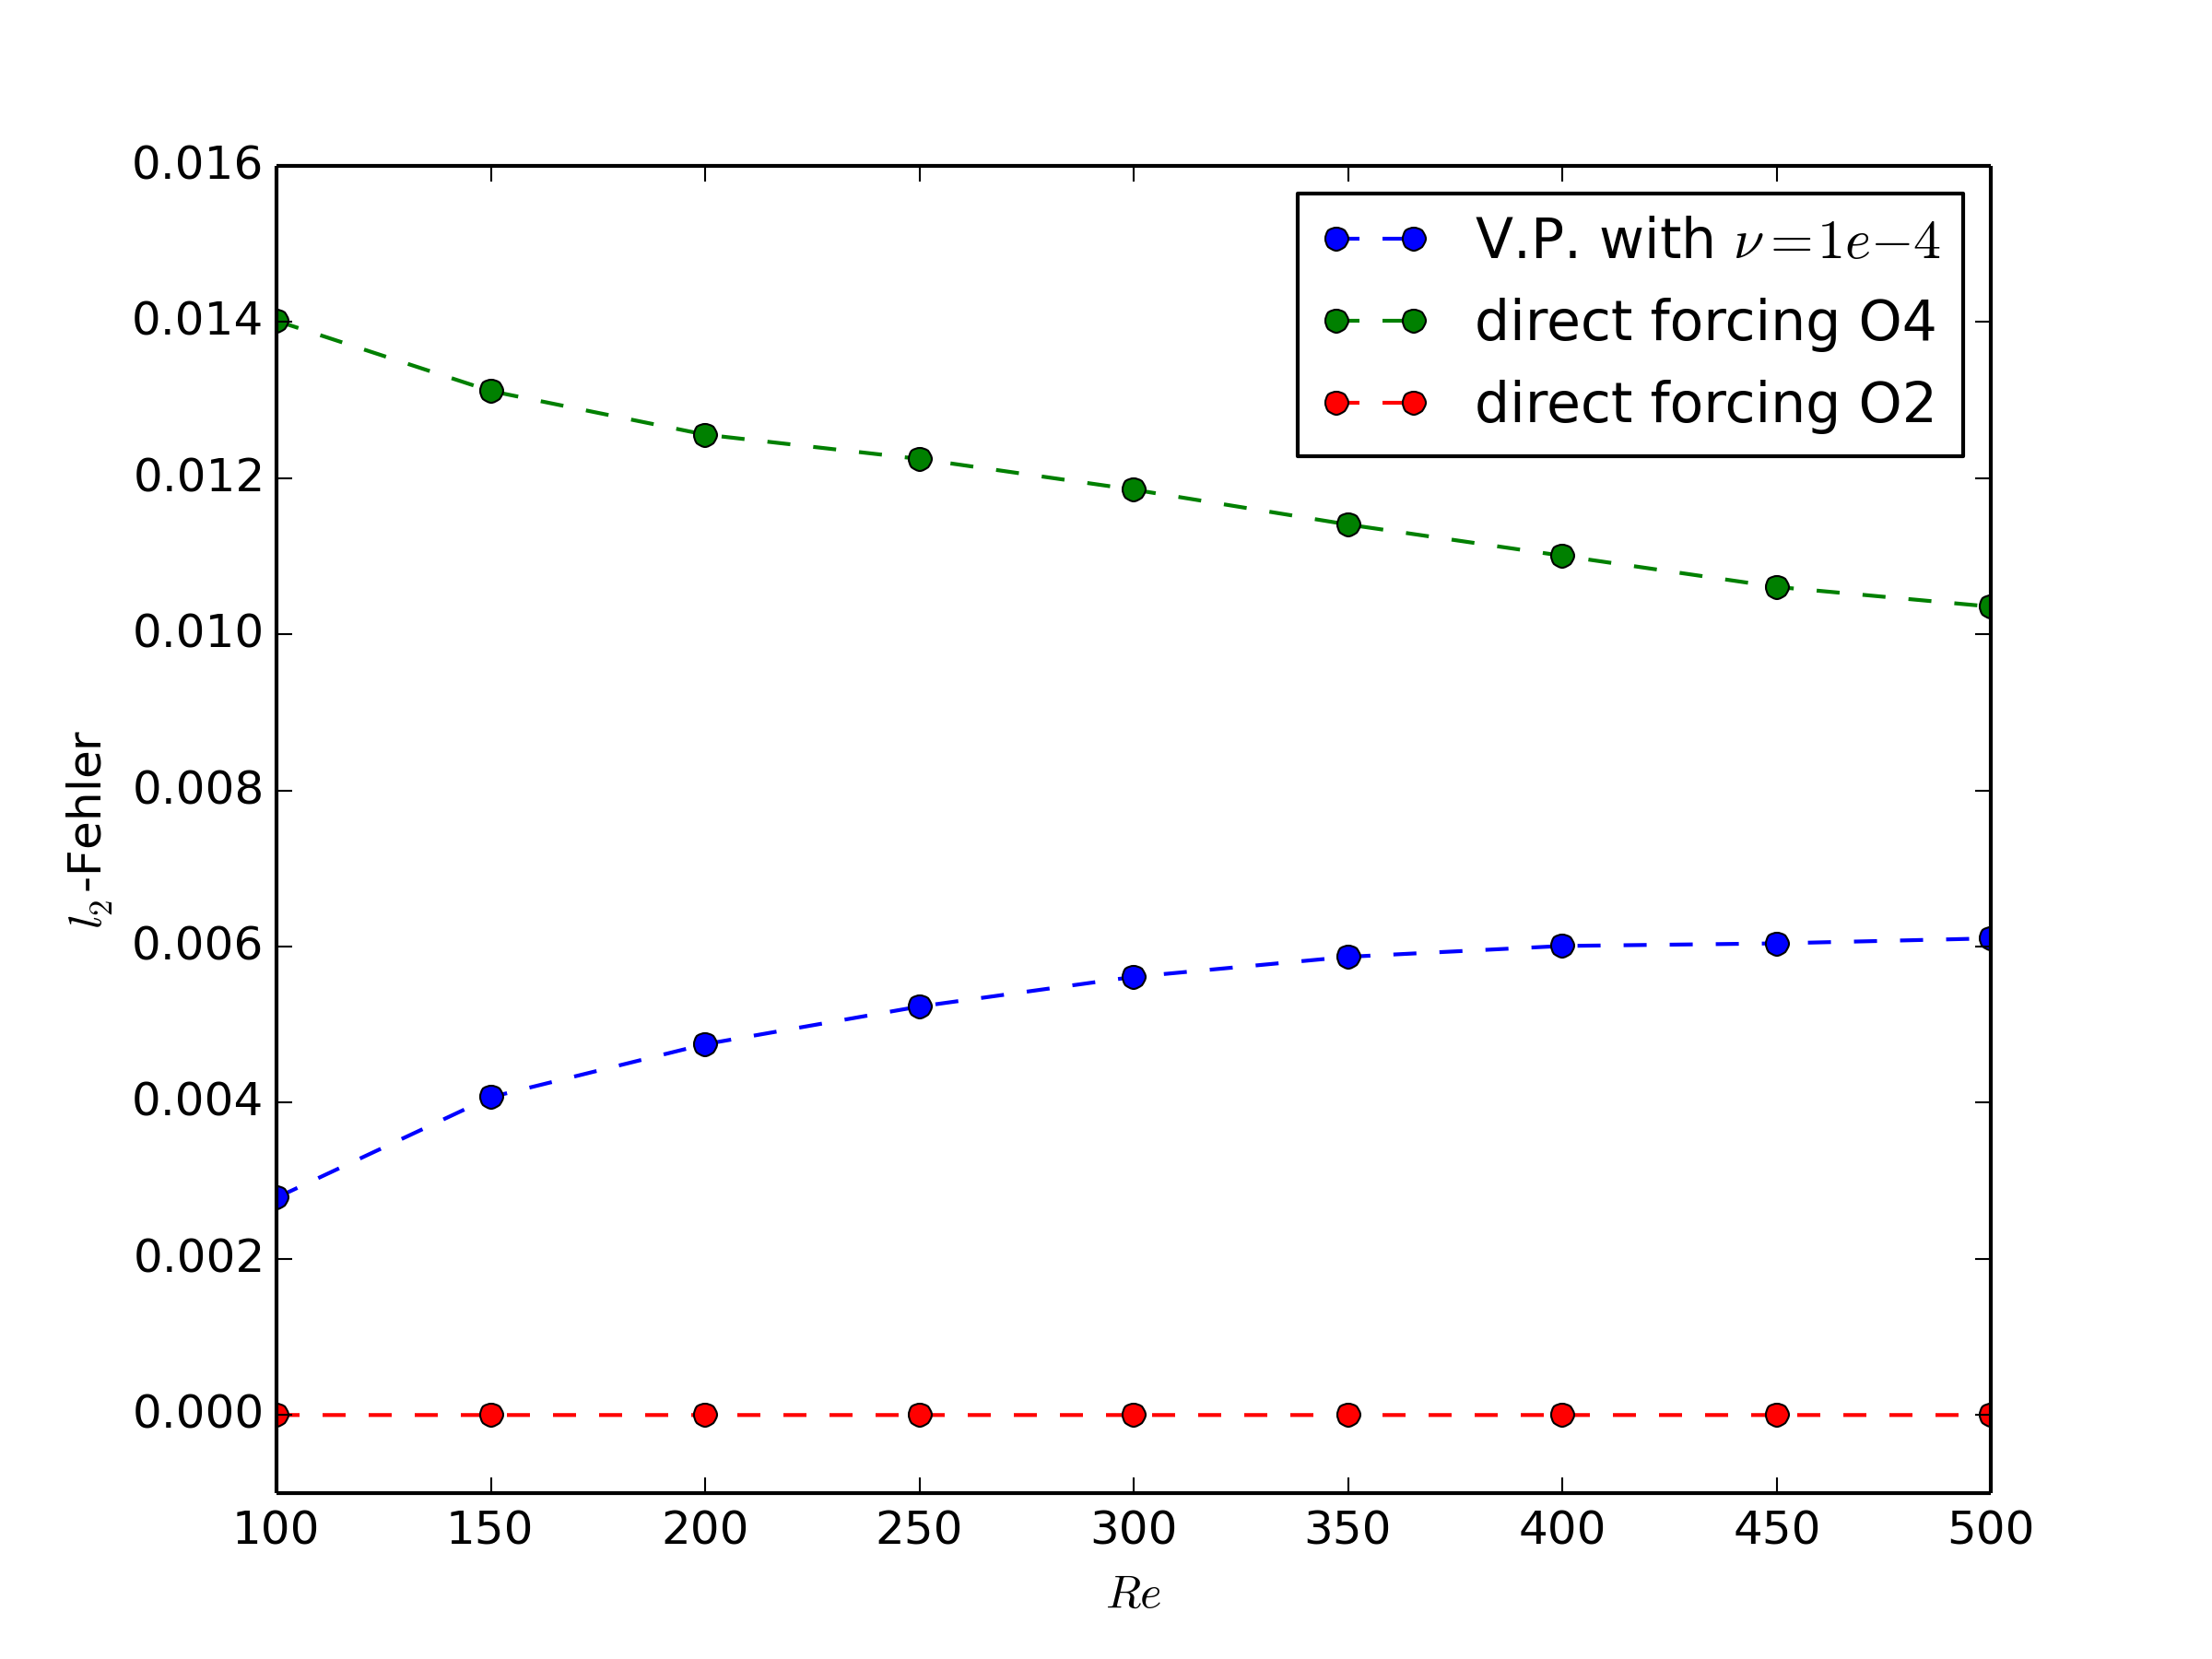
\includegraphics[width=0.6\textwidth]{gfx/immersed_boundary_methods/dfo2o4.png}\label{fig:df_o2o4}
  \caption{bla}
\end{figure}

-Zeitserie

-einleitung gekrümmte geometrien

\subsection{Direct Forcing mit Volume Fraction}
-paper quote formeln
-implementierung beispiel

\section{Direct Forcing mit Interpolation}
-paper quote formeln
-implementierung beispiel

\section{Methoden-Vergleich und numerische Validierung}
In diesem Abschnitt sollen die verschiedenen Methoden über numerische Testfälle validiert und miteinnander
verglichen werden.


\subsubsection{Poiseuille Strömung im Zylinder}

\subsubsection{Zusammenfassung}


\subsection{No-Flux-Boundaries}

\subsubsection{'Variable Konduktivität'}










